\section{Christmas Break}

\subsection*{Overview:}
This Festive break has not just been relaxing, but also hugely beneficial for my EPQ. Over just I couple a weeks I have  conducted research and produced practical demos into every aspect of my project.


\subsection*{Achievements, Thoughts and Ideas:}
I started by further communicating with my summer internship manager about the technical 'stack' they use for their tools, having spent a week learning from the team previously I knew this would benefit my projects by being a 'resilient, expandable and professional' system on which to build my artifact.

\begin{figure}[H]
    \centering
    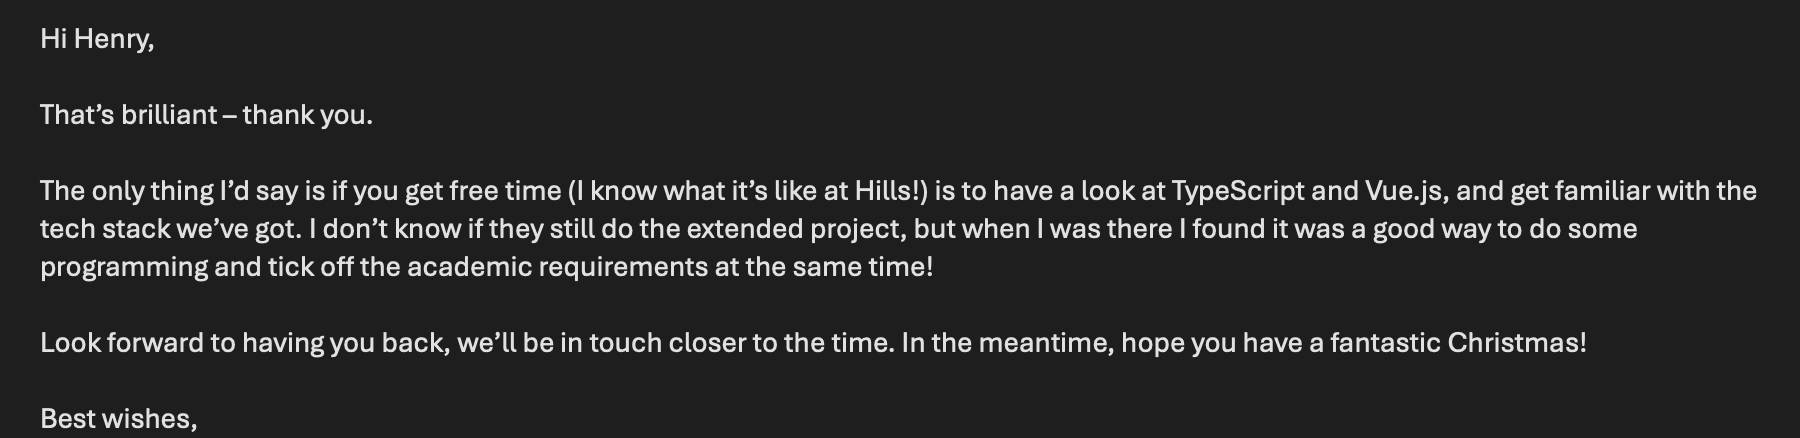
\includegraphics[width=0.8\textwidth]{Diary/12_ChristmasBreak/media/emailFromInternship.png}
    \caption{Email from summer internship manager (and an endorsement for the EPQ program :)}
\end{figure}

From these conversations (alongside further research) I then decided on using a web framework called Vue JS to produce my artifact. Until this point My Flask app had been handling both the backend data storage as well as serving 'static' html pages to the user, in short, when a user went to my website their browser would load a single page, should they the want to see different content (such as user settings) the browser would request and load a separate page (in the same way it would should I user change website from google.com to micrsoft.com etc). Using Vue however, the same web page dynamically updates the content shown making the site a) faster b) work fully offline and c) easier to manage as a developer. The added beauty of VUE Js is that none of my current website code gets replaced, instead it is simply rolled into a new layout and iterated upon, my python code also remains the same an now servers only as the backend server which the frontend Vue app will communicate with whenever the user commits a change.

With an underlying framework chosen I now wanted to work on creating an aesthetic and intuitive user experience. I knew in the scope of the EPQ I wouldn’t have time to create this from scratch so I looked to leverage a library of components whilst my full findings can be found here, while I couldn’t find any library which met my exact needs I learnt of methods to use these as a template and produce my own 'components' on top of these 'cores'. After researching many options I settled on Shadcdn for its widespread support, powerful features and most importantly, ability to be fully adapted and changed to fit my use case

Alongside the Frontend redesign I also had to make some tweaks to my flask server backend. Mostly this primarily involved removing code that was used to return webpages at routes such as domain.com/home and domain.com/note1 etc. My python code is therefore looking much neater now.

Having now started prototyping some integrated Vue webapps I was finding issues with my current code backup technique of OneDrive sync. Professional tools such as Vue often utilise CLI (command line interface) tools for installing packages (pieces of code that can be 'plugged in' to my software providing common features rather than continually remaking them from scratch), while these tools are incredibly powerful (installing and keeping many files compatible and up to date etc) OneDrive sometimes struggles to sync many hundreds of files added at the same time, this results in issues when trying to access code from other devices and attempts to fix the issues (e.g. recreating 'lost' files) causes further sync issues when the original file Is finally spotted by OneDrive and a duplicate now exists. This annoying slowdown in productivity finally prompted me to learn the industry standard (and truly reliable) world of GIT. GIT is a system for tracking code changes through a variety of 'branches'. By keeping a central repository hosted on GitHub(.com),  whenever I make a change on my local client and 'commit it' the change gets 'pulled' through to the master online copy alongside any comments I make. Alongside the benefits of reliable online backups, GIT also fully tracks versions of code and changes made over time such that should I make a mistake that later causes a headache I can go back through the timeline, spot the issue and easily solve it. Prior to this I had been using a highly inefficient system of making a new file for each major revision and I'm thankful to now be using a proper system for this.

\subsection*{What went well?}

I am now feeling very prepared to build my final artefact project using industry standard and 'battle tasted' tools which will help me achieve goals

\subsection*{Plans for next week:}

Next week I have some graphing changes to be made and I want to collect some primary research which will help inform my project design decisions
